\chapter{Efficient Learning and Unlearning via Large-Scale Conditional Independence Testing} \label{chap:lcodec} 

While from one perspective we may be able to constrain our parameter space to one which is desirable,
it may be the case that we cannot
affect or intervene in the model prior to training.
In these cases, 
we may still wish to identify a \textit{subset of existing parameters} that are important or related to particular samples or sample subsets.
As personal data becomes a valuable commodity, legislative efforts have begun to push back on its widespread collection/use particularly for training ML models. Recently, a focus is the ``right to be forgotten" (RTBF), i.e., the right of an individual's data to be deleted from a database (and derived products).
Despite existing legal frameworks on fair use, industry scraping has led to personal images being used without consent, e.g. \citep{Exposing}.
Large datasets are not only stored for descriptive statistics, but used in training large models.
While regulation (GDPR, CCPA) has not specified the extent to which data must be forgotten, it poses a clear question: is  deletion of the data enough, or does a model trained on that data also needs to be updated?

Recent work by \citep{carlini2019secret,carlini2020attack} has identified scenarios where trained models are vulnerable to attacks that can reconstruct input training data. More directly, recent rulings by the Federal Trade Commission \cite{ftc,ftc2} have ordered companies to fully delete and destroy not only data, but also any model trained using those data.
While deletion and (subsequent) full model retraining without the deleted samples is possible, most in-production models require weeks of 
training and review, with extensive computational/human resource cost. With additional deletions, it is infeasible to retrain each time a new delete request comes in. 
% So, are there updates to the model that ensure the data has been deleted (or at least approximately deleted), and full retraining can be postponed?
% Existing works have answered this question in the affirmative, but the computational burden has limited their broad use.
So, how to update a model ensuring the data is deleted without retraining?

\textbf{Task.} Given a set of input data $\cS: \{z_i\}_{i=1}^n \sim \mathcal{D}$ of size $n$, training simply identifies a hypothesis $\hat{w} \in \cW$  via an iterative scheme $w_{t+1} = w_t - g(\hat{w},z')$ until convergence, where $g(\cdot,z')$ is  a stochastic gradient of a fixed loss function. Once a model at convergence is found, \textit{machine unlearning} aims to identify an update to $\hat{w}$ through an analogous \textit{one-shot unlearning update}:
\begin{align}\label{eq:unlearn}
    w' = \hat{w} + g_{\hat{w}}\left(z'\right),
\end{align}
for a \textit{given} sample $z' \in \cS$ that is to be \textbf{unlearned}.
%While forms of $g(z')$ have {\color{red}been recently been identified \cite{abc}}, practically they remain infeasible because a complete Hessian computation and inversion is needed. 

\begin{figure*}
	\centering
	% 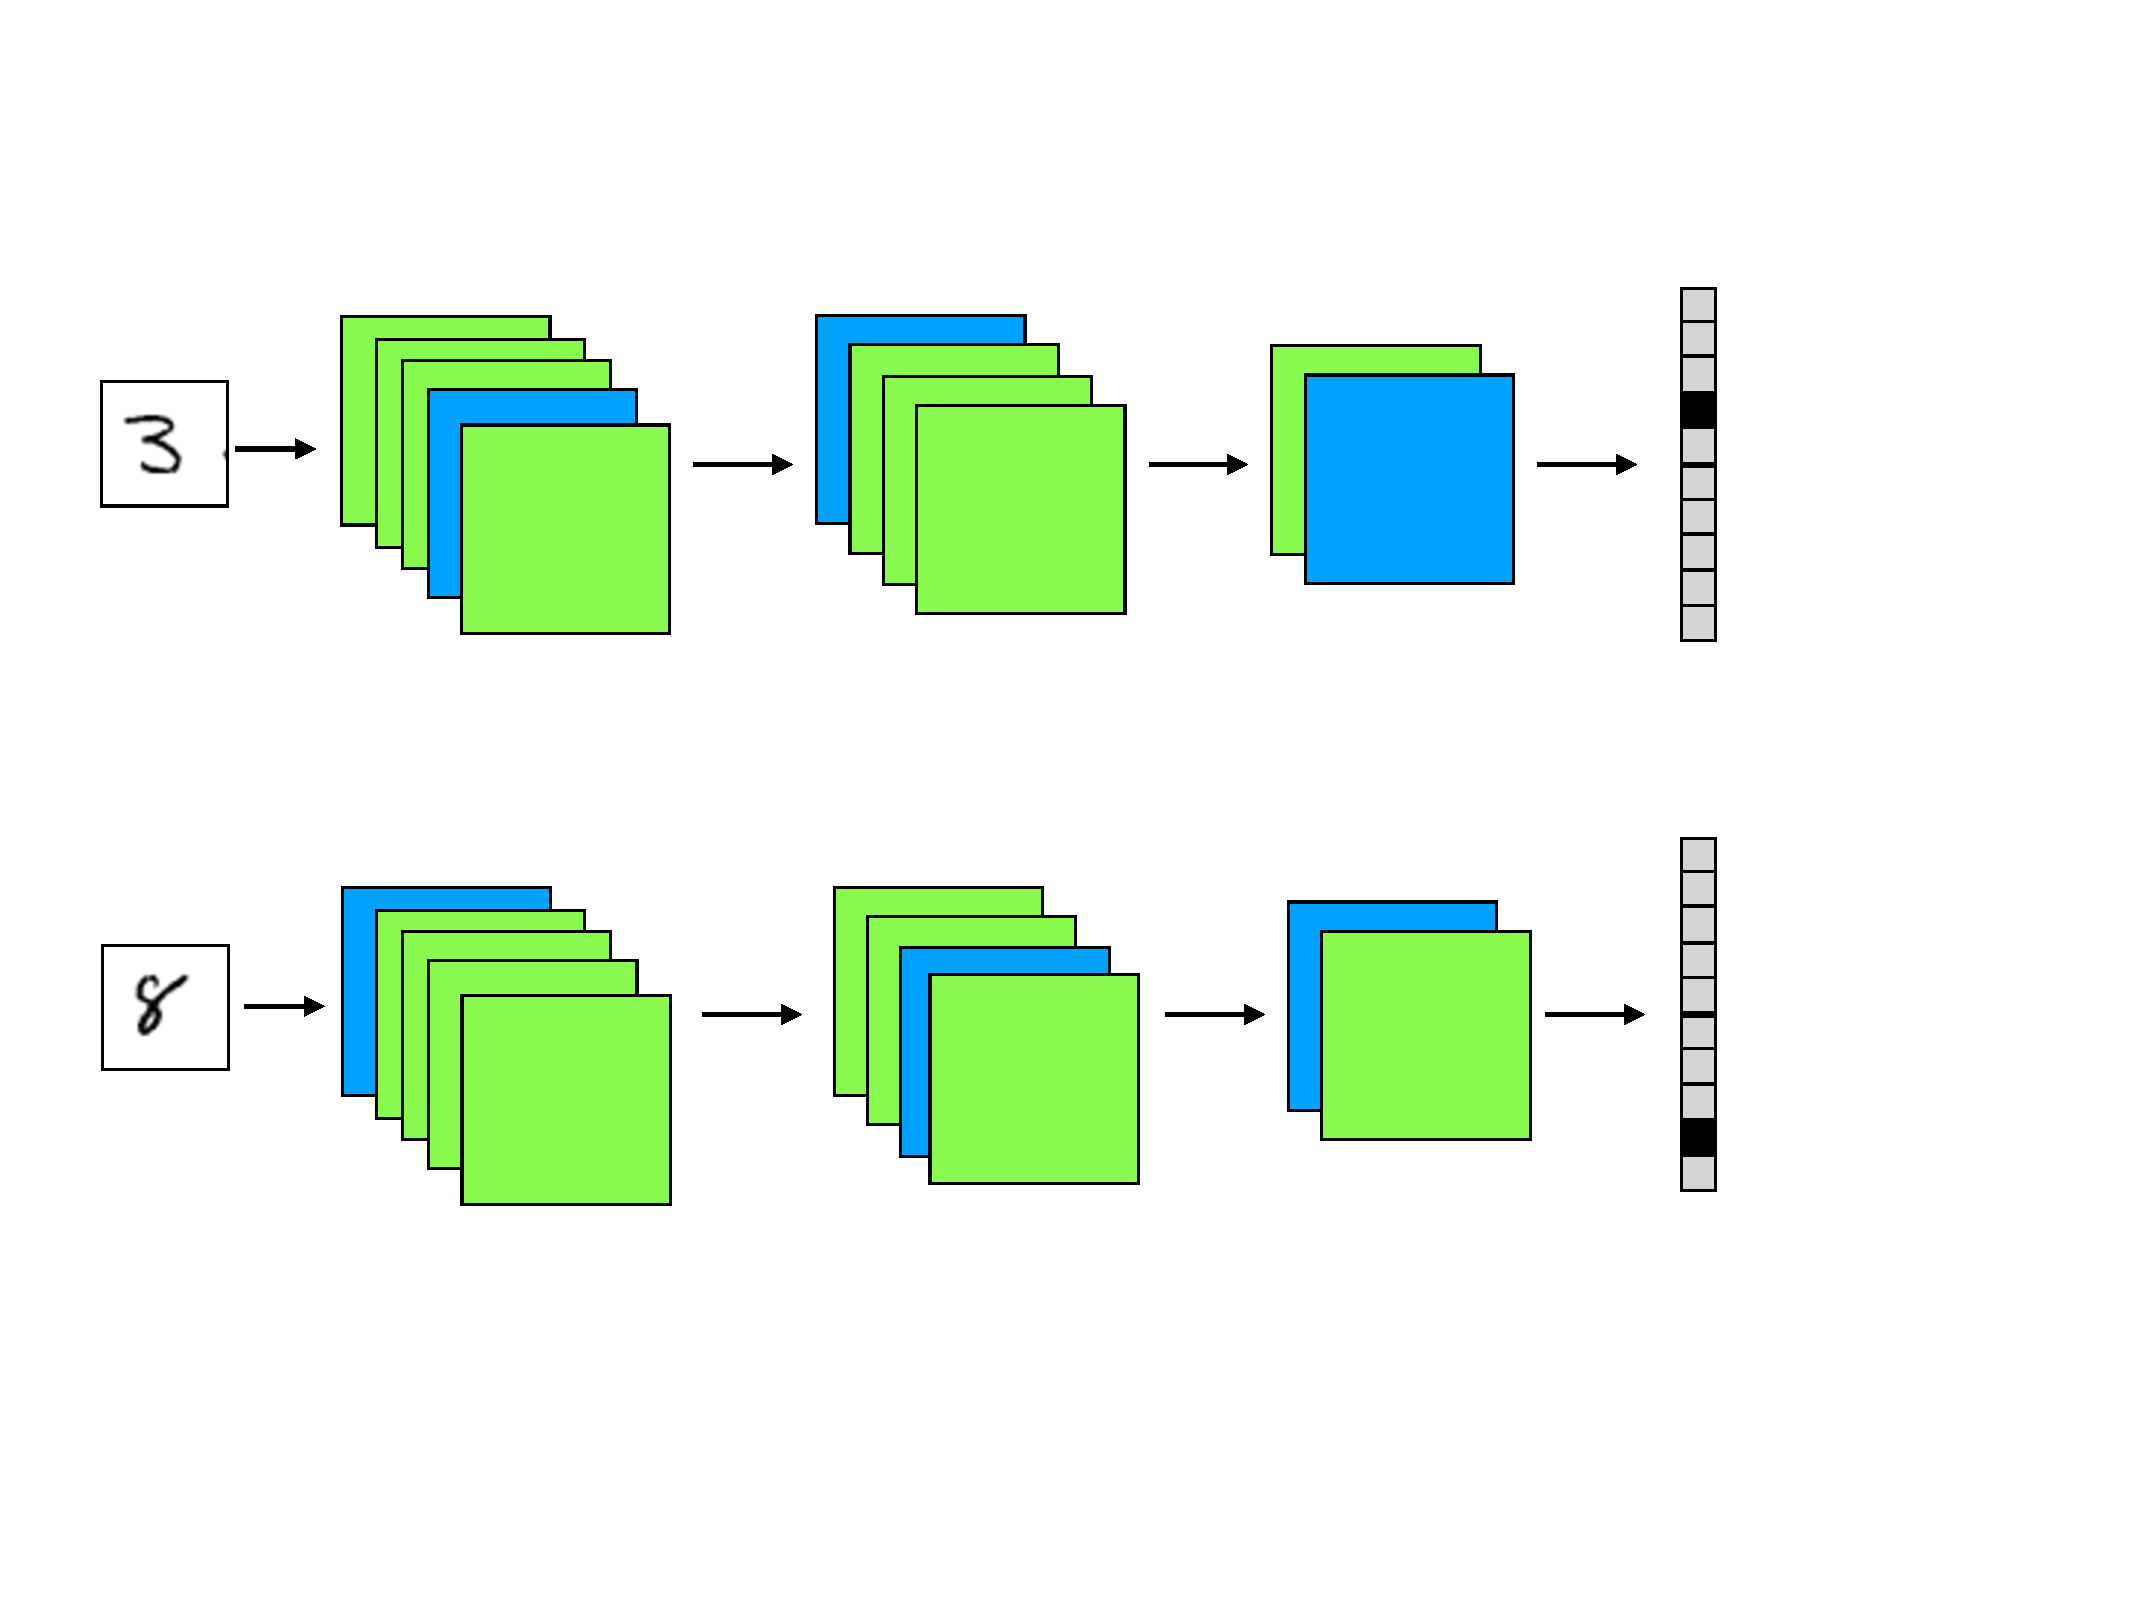
\includegraphics[height=1.5in,trim={1.5cm 5cm 3cm 3.5cm},clip]{figs/layercnn.pdf}
	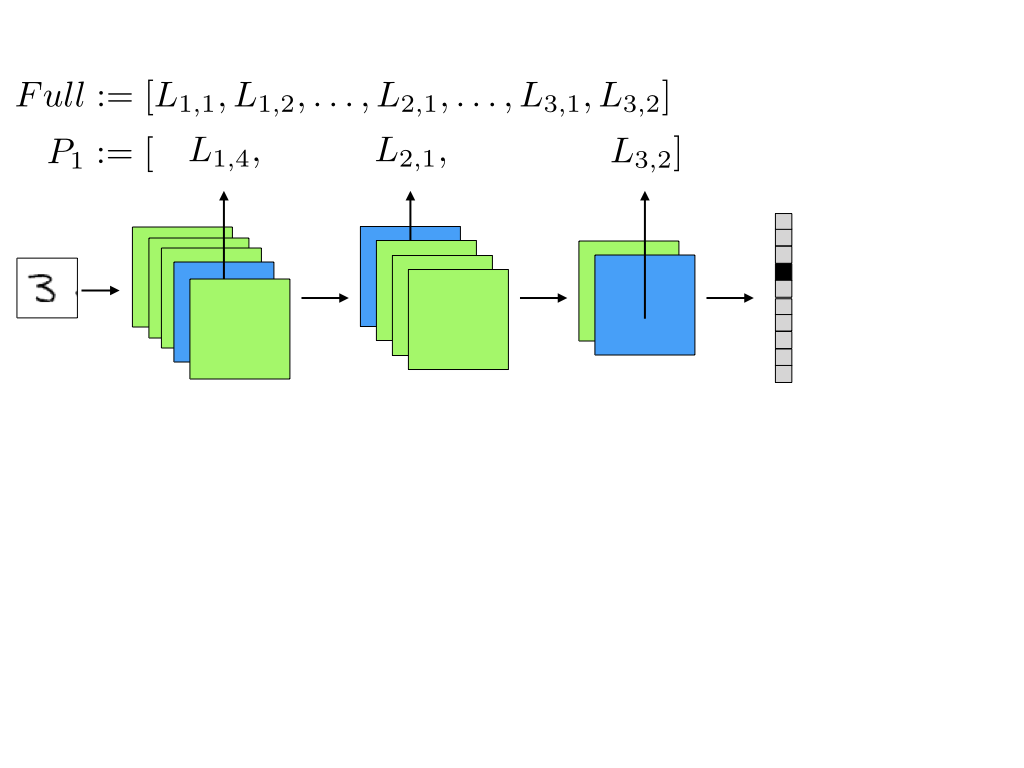
\includegraphics[width=0.48\columnwidth,trim={0cm 12cm 5cm 2.5cm},clip]{chap4/layercnn.png}
	%\includegraphics[height=2in,trim={7cm 8cm 9cm 7.7cm},clip]{figs/new.pdf}
	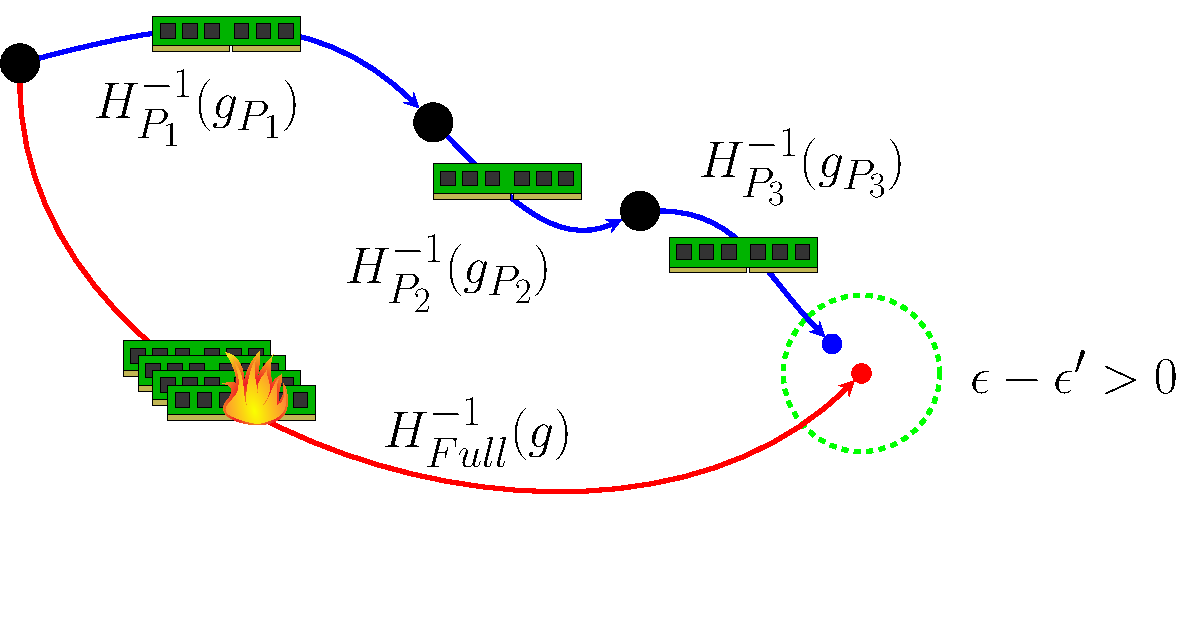
\includegraphics[width=0.48\columnwidth,trim={0cm 1cm 0cm 0cm},clip]{chap4/unlearning_fig.pdf}
	\caption{\label{fig:main}Large deep learning networks typically associate specific subsets of network parameters, blocks (blue), to specific samples in the input space.
		Traditional forward or backward passes may not reveal these blocks: high correlations among features may not distinguish important ones. Input perturbations can be used to identify them in a probabilistic, distribution-free manner. These blocks can then be unlearned together in an efficient block-coordinate style update (right, blue lines), approximating an update to the full network which requires a costly/infeasible full Hessian inverse (red line).}
\end{figure*}

Let $\cA$ be an algorithm that takes as input a training set $\cS$ and outputs a hypothesis $w \in \cW$, defined by a set of $d$ parameters $\Theta$. 
An unlearning scheme $\cU$ takes as input a sample $z' \in \cS$ used as input to $\cA$, and ideally, outputs an {\bf updated} hypothesis $w' \in \cW$ where $z'$ has been deleted from the model.
%
% Clearly within unlearning we do not wish to simply rerun $\cA$ on the subset without the sample to delete.
% Particularly for modern machine learning problems with extremely large datasets and model architectures, retraining can be costly or impossible.
%
% Retraining may be costly or impossible, but provides a baseline oracle to which we can compare updates as in \eqref{eq:unlearn}.
% However, this provides a baseline with which we can compare any other potential unlearning algorithm to.
% Namely, a
An unlearning algorithm should output a hypothesis that is close or equivalent to one that would have been learned had the input to $\cA$ been $\cS \setminus z^\prime$. A framework for this goal was given by \cite{ginart2019making} as,
% Following \cite{sekhari2021remember}, 
\begin{definition}[$(\epsilon,\delta)-$ forgetting]\label{def:forget}
	For all sets $\cS$ of size $n$, with a ``delete request'' $z' \in \cS$, an unlearning algorithm $\cU$ is $(\epsilon, \delta)-$forgetting if
	\begin{align}
	\PP(\cU(\cA(S), z') \in \cW) \leq e^\epsilon\PP(\cA(\cS\setminus z') \in \cW) + \delta
	\end{align}
\end{definition}
In essence, for an existing model $w$, a good unlearning algorithm for request $z' \in \cS$ will output a model $\hat{w}$ close to the output of $\cA(S \setminus z')$ with high probability.

\begin{remark}
	Definition \ref{def:forget} is similar to the standard definitions of differential privacy. The connection to unlearning is: if an algorithm is $(\epsilon, \delta)-$forgetting for unlearning, then it is also differentially private. 
\end{remark}

%\cite{unlearning} provide a straightforward algorithm for mild assumptions under the structure of the algorithm $\cA$.
If $\cA$ is an empirical risk minimizer for the loss $f$, let
\begin{align}
\cA : (\cS, f) \rightarrow \hat{w}%, \nabla^2 F(\hat{w}),
\end{align}
$\hat{w} = \arg\min F(w)$ and $F(w) = \frac{1}{n}\sum_{i=1}^n f(w, z_i).$ 
%$\nabla^2 F(\hat{w})$ is the Hessian of the empirical loss at the minimizer $\hat{w}$.
% Ideally, we would like to perform a ``one-shot" update to $\hat{w}$, in the same way we may update model parameters in a traditional forward learning setting. Consider the following \textit{one-shot unlearning update}:
% \begin{align}\label{eq:bbunlearn}
% \tilde{w} = \hat{w} + g(z^\prime).
% \end{align}
Recall $g(z')$ from \eqref{eq:unlearn}:  
our unlearning task 
essentially involves 
identifying 
the form of $g(z')$ for which the update in \eqref{eq:unlearn} is $(\epsilon,\delta)$-forgetting. If an oracle provides this information, we have 
accomplished the unlearning task.

The difficulty, 
as expected, tends to 
depend on $f$ and $\cA$. 
Recent unlearning results have identified forms of $f$ and $\cA$ where such a $g(z')$ exists. The authors in \citep{sekhari2021remember} define $g(z') = \frac{1}{n-1}H'^{-1}\nabla f(\hat{w},z')$, where
%Given this, they provide an unlearning algorithm $\cU$ with the update for each $z \in T$:
\begin{align}\label{eq:sekhariunlearn}
H' &= \frac{1}{n-1} \left(n\nabla^2 F(\hat{w}) - \nabla^2 f(\hat{w},z')\right),
%    \bar{w} &= \hat{w} + \frac{1}{n-1} (\hat{H})^{-1} \nabla f(\hat{w},z) \\
%    \tilde{w} &= \hat{w} + N(0,\sigma^2 I)
\end{align}
with additive Gaussian noise $w' = w' + N(0,\sigma^2)$ scaling as a function of $n, \epsilon, \delta$, and the Lipschitz and (strong) convexity parameters of the loss $f$. We can interpret the update using \eqref{eq:sekhariunlearn} from the optimization perspective as a trajectory ``reversal": starting at a random initialization, the first order (stochastic gradient) trajectory of  ${w}$ (possibly) {\em with}  $z'$ is reversed using {\em residual} second order curvature information (Hessian) at the optimal $\hat{w}$ in \eqref{eq:sekhariunlearn}, achieving unlearning. This is shown to satisfy Def.~\ref{def:forget}, and only incurs an additive error that scales by $O(\sqrt{d}/n^2)$ in the gap between $F(w')$ and the global minimizer $F(w^*)$ over the ERM $F(\hat{w})$. 

% \ronak{perhaps a note on Laurens CR paper: requiring DP-trained model while Sekhari does not, bounding population risk as opposed to residual empirical results}

%Indeed, such a Newton step for unlearning has been evaluated in practice, in a slightly different form, by \cite{certified}. 
\textbf{Rationale for approximate schemes.} From the reversal of $w$ optimization perspective, it is clear that there may be other choices to achieve unlearning.
%The aforementioned update requires storing, computing, and inverting the $O(d^2)$ Hessian matrix.
For a practitioner interested in unlearning, the aforementioned algorithm (as in \eqref{eq:sekhariunlearn}) can be directly instantiated if one has extensive computational resources.
Indeed, in settings where it is not directly possible to compute the Hessian inverse necessary for $H'^{-1} \nabla f(\hat{w},z')$, we must consider alternatives. 

\textbf{A potential idea.} Our goal is to identify a form of $g(z')$ that \textbf{approximates} $H'^{-1} \nabla f(\hat{w},z')$. 
Let us consider the Newton-style update suggested by 
\eqref{eq:sekhariunlearn}
as a smoothing of a traditional first order gradient step. 
The inverse Hessian is a weighting matrix, appropriately scaling the gradients based on the second order difference between the training set mean point $F(\hat{w})$ and at the sample of interest $f(\hat{w},z')$. 
This smoothing can also be seen from an information perspective: the Hessian in this case corresponds to a Fisher-style information matrix, and its inverse as a conditional covariance matrix \citep{Golatkar_2021_CVPR,golatkar2020forgetting}.
It is not hard to imagine that from this perspective, if there are \textit{specific set of parameters} that have \textit{small gradients} at $f(\hat{w},z')$ or if the information matrix is zero or small, then we need not consider their effect. 


\textbf{Contributions.} We will address several computational issues with existing approximate formulations for unlearning by taking advantage of a new statistical scheme for sufficient parameter selection. 
First, in order to ensure that a sample's impact on the model predictions is minimized, we propose a measure for computing conditional independence called L-CODEC which  identifies the Markov Blanket of parameters to be  updated. 
% Extending hypercolumn activations, we identify neural network parameter subsets that are sufficient for model scrubbing.
Second, we will show that the L-CODEC identified Markov Blanket enables unlearning in previously infeasible deep models, scaling to networks with hundreds of millions of parameters. 
%{\color{red} with graceful performance degradation}.
Finally, we will demonstrate the ability of L-CODEC to unlearn samples and entire classes on networks, from CNNs/ResNets to transformers, including face recognition and person re-identification models.